%% Layout of the Lyra discriminator v1 model
%% Author: Dominik Haspel
\documentclass[border=0pt]{standalone}





%% Load the required libraries
\usepackage{amsmath}
\usepackage{xcolor}
\usepackage{tikz}
\usepackage{tensor}





%% Setup the tikz library
\usetikzlibrary{shapes,arrows,decorations.markings} % for arrow heads
\usetikzlibrary{shadows}
\usetikzlibrary{positioning}

\tikzstyle{single} = [draw, fill=white!20, rectangle, thick, align=center]
\tikzstyle{stack} = [single, double copy shadow={shadow xshift=1.5pt, shadow yshift=1.5pt}]
\tikzstyle{block} = [single, double distance=1pt]

\tikzstyle{conn} = [->,thick]
\tikzstyle{connstack} = [conn,shorten >=3pt]

\tikzstyle{vecArrow} = [dash pattern={on 2pt off 1pt}, thick, decoration={markings,mark=at position
   1 with {\arrow[semithick]{open triangle 60}}},
   double distance=1.4pt, shorten >= 5.5pt,
   preaction = {decorate},
   postaction = {draw,line width=1.4pt, white,shorten >= 4.5pt}]





%% Define custom colors
\definecolor{cnnDefault}{rgb}{0,0,0}
\definecolor{cnnActivation}{rgb}{1.0,0,0}
\definecolor{cnnDimension}{rgb}{0,0,1.0}
\definecolor{cnnFeature}{rgb}{0,0.7,0}

\newcommand{\colorDefault}[1]{{\color{cnnDefault}#1}}
\newcommand{\colorActivation}[1]{{\color{cnnActivation}#1}}
\newcommand{\colorDimension}[1]{{\color{cnnDimension}#1}}
\newcommand{\colorFeature}[1]{{\color{cnnFeature}#1}}





%% Define custom commands
\newcommand{\nntensor}[5]{
	$\tensor*[^{#1\;}_{#3\;}]{\text{#5}}{^{\;#2}_{\;#4}}$
}
\newcommand{\nninput}[2][]{
	\nntensor{}{\color{cnnDimension}#2}{}{\color{cnnFeature}#1}{i}
}
\newcommand{\nnconcat}[2][]{
	\nntensor{}{\color{cnnDimension}#2}{}{\color{cnnFeature}#1}{cc}
}
\newcommand{\nnreshape}[2][]{
	\nntensor{}{\color{cnnDimension}#2}{}{\color{cnnFeature}#1}{r}
}
\newcommand{\nnconv}[6][1]{
	\nntensor{#2,#3}{{\color{cnnDimension}#4}}{{\color{cnnActivation}#6}}{{\color{cnnFeature}#5}}{c#1}
}
\newcommand{\nninception}[4][]{
	\nntensor{#1}{{\color{cnnDimension}#2}}{{\color{cnnActivation}#4}}{{\color{cnnFeature}#3}}{Inception}
}
\newcommand{\nnflatten}[2][]{
	\nntensor{}{{\color{cnnDimension}#2}}{#1}{}{f}
}
\newcommand{\nndense}[3][]{
	\nntensor{}{{\color{cnnDimension}#2}}{{\color{cnnActivation}#3}#1}{}{d}
}
\newcommand{\nnoutput}[3][]{
	\nntensor{}{{\color{cnnDimension}#2}}{{\color{cnnActivation}#3}#1}{}{o}
}





\begin{document}





%% Display neural net layout
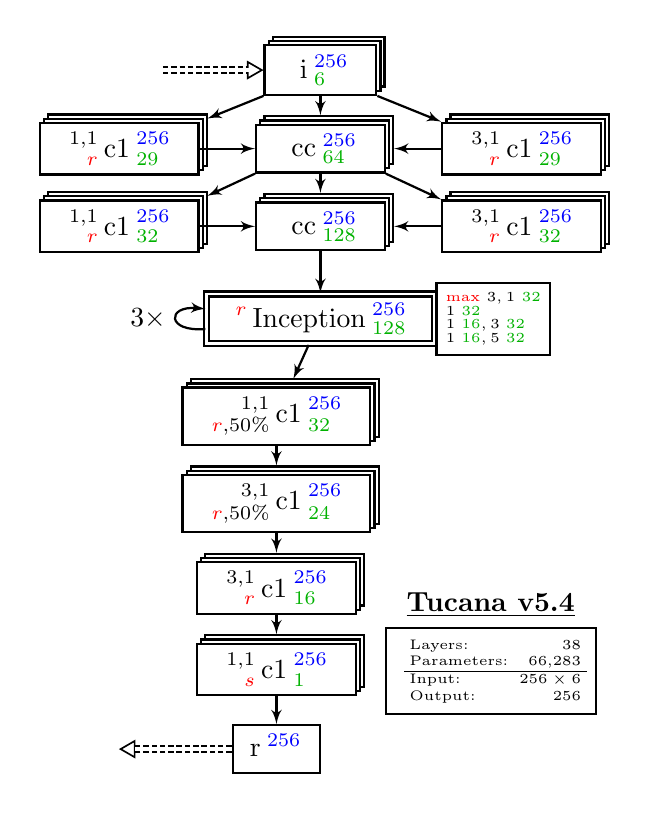
\begin{tikzpicture}[auto, node distance=1em and 2em, >=latex']

	%% Display input and mask
	\node[stack] (data) {\nninput[6]{256}};
	\draw[vecArrow] ++(-2,0) to (data);

	%% Display feature preparation stem
	\node[stack, below=of data] (data2) {\nnconcat[64]{256}};
	\node[stack, right=of data2] (conv1) {\nnconv[1]{3}{1}{256}{29}{r}};
	\node[stack, left=of data2] (recombine1) {\nnconv[1]{1}{1}{256}{29}{r}};
	\draw[connstack] (data) -- (data2);
	\draw[connstack] (data.south west) -- (recombine1.north east);
	\draw[conn] (data.south east) -- (conv1.north west);
	\draw[conn] (recombine1) -- (data2);
	\draw[connstack] (conv1) -- (data2);

	\node[stack, below=of data2] (data3) {\nnconcat[128]{256}};
	\node[stack, right=of data3] (conv2) {\nnconv[1]{3}{1}{256}{32}{r}};
	\node[stack, left=of data3] (recombine2) {\nnconv[1]{1}{1}{256}{32}{r}};
	\draw[connstack] (data2) -- (data3);
	\draw[connstack] (data2.south west) -- (recombine2.north east);
	\draw[conn] (data2.south east) -- (conv2.north west);
	\draw[conn] (recombine2) -- (data3);
	\draw[connstack] (conv2) -- (data3);

	%% Display the inception layers
	\node[block, below=1.5em of data3] (inception) {\nninception[\colorActivation{r}]{256}{128}{}} edge [conn, in=175, out=185, loop, looseness=5] node {$3\times$} (inception);
	\node[single, right=0em of inception, align=left] (inceptionParam) {
		\tiny $\colorActivation{\max}~3,1~\colorFeature{32}$ \\[-0.7em]
		\tiny $1~\colorFeature{32}$ \\[0-0.7em]
		\tiny $1~\colorFeature{16},3~\colorFeature{32}$ \\[0-0.7em]
		\tiny $1~\colorFeature{16},5~\colorFeature{32}$
	};
	\draw[conn] (data3) -- (inception);

	%% Display the final logics layers
	\node[stack, below left=1.5em and -6em of inception] (reduce) {\nnconv[1]{1}{1}{256}{32}{r\colorDefault{,50\%}}};
	\draw[connstack] (inception) -- (reduce);
	\node[stack, below=of reduce] (final1) {\nnconv[1]{3}{1}{256}{24}{r\colorDefault{,50\%}}};
	\draw[connstack] (reduce) -- (final1);
	\node[stack, below=of final1] (final2) {\nnconv[1]{3}{1}{256}{16}{r}};
	\draw[connstack] (final1) -- (final2);
	\node[stack, below=of final2] (final3) {\nnconv[1]{1}{1}{256}{1}{s}};
	\draw[connstack] (final2) -- (final3);
	\node[single, below=of final3] (output) {\nntensor{}{\colorDimension{256}}{}{}{r}};
	\draw[conn] (final3) -- (output);
	\draw[vecArrow] (output) to ++(-2,0);

	%% Draw title, statistics and in/out vectors	
	\node[single, below right=-2.5em and 1em of final3] (stats) {\setlength{\tabcolsep}{2pt}\renewcommand{\arraystretch}{0.5}
	\begin{tabular}[h!]{lr}
		\tiny Layers: & \tiny 38 \\
		\tiny Parameters: & \tiny 66,283 \\
		\hline
		\tiny Input: & \tiny $256 \times 6$ \\
		\tiny Output: & \tiny $256$ \\
	\end{tabular}};

	\node[above=0em of stats] (title) {\underline{\bf Tucana v5.4}};

	\path
    ([shift={(-10\pgflinewidth,-10\pgflinewidth)}]current bounding box.south west)
    ([shift={( 15\pgflinewidth, 15\pgflinewidth)}]current bounding box.north east);
\end{tikzpicture}





\end{document}